% !TeX root = ../../main.tex
\begingroup
\ChSixBegin
\emergencystretch=2em
\chapter{Reconstructing Sepsis Trajectories from Clinical Case Reports using LLMs: the Textual Time Series Corpus for Sepsis}\label{chap:ch06}
\noindent\emph{This chapter is based on:} \cite{pmlr-v333-noroozizadeh26a}.\par\smallskip

% % !TeX root = ../../../../main.tex
\begin{ChSixAbstract}
Clinical case reports and discharge summaries may be the most complete and accurate summarization of patient encounters, yet they are finalized, \emph{i.e.}, timestamped after the encounter.
Complementary structured data streams become available sooner but suffer from incompleteness.
To train models and algorithms on more complete and temporally fine-grained data, we construct a pipeline to phenotype, extract, and annotate time-localized findings within case reports using large language models.
We apply our pipeline to generate an open-access textual time series corpus for Sepsis-3 comprising 2,139 case reports from the PubMed-Open Access (PMOA) Subset.
To validate our system, we apply it to PMOA and timeline annotations from i2b2/MIMIC-IV and compare the results to physician-expert annotations.
We show high recovery rates of clinical findings (event match rates: GPT-5--0.93, Llama 3.3 70B Instruct--0.76) and strong temporal ordering (concordance: GPT-5--0.965, Llama 3.3 70B Instruct--0.908). 
Our work characterizes the ability of LLMs to time-localize clinical findings in text, illustrating the limitations of LLM use for temporal reconstruction and providing several potential avenues of improvement via multimodal integration.
\end{ChSixAbstract}


\ChSixParagraph{Data and Code Availability}
This paper uses the i2b2 \citep{sun2013evaluating}, MIMIC-IV \citep{ch06:johnson2023mimic}, and PubMed Open Access (PMOA) datasets \citep{pmc2024open}, as well as the timeline annotations from \cite{ch06:frattallone2024using}.
Code and annotations are available at: \url{https://github.com/Shahriarnz14/T2S2}.

\ChSixParagraph{Institutional Review Board (IRB)}
This research has been designated by our IRB as Not Human Subjects Research.


% !TeX root = ../../../../main.tex
\subsection{Textual Time Series corpus for Sepsis (T2S2): Sepsis-Specific Reconstruction Case Study}
\label{ch06:sec:intro}

The Third International Consensus Definitions for Sepsis (Sepsis-3) are the benchmark definitions for sepsis, the dysfunctional immune response to an infection, which are used in trial eligibility criteria \citep{kyriazopoulou2021procalcitonin} and phenotyping studies \citep{ch06:seymour2019derivation}.
In the critical care literature, sepsis is seen as a heterogeneous disease, a pathway arrived upon from a multitude of infectious origins, anatomical sites, and comorbid profiles.  
There is increasing recognition of the importance of time in understanding sepsis and sepsis progression, as seen in early-warning systems \citep{henry2022factors}, variation in prediction utility \citep{kamran2024evaluation}, and endotype characterization \citep{ch06:noroozizadeh2023temporal}.

Meanwhile, structured data streams, which are the data resources these tools use, are often incomplete records with insufficient information to render or confirm a diagnosis of sepsis \citep{moldwin2021empirical}. %
A more complete alternative is the discharge summary, or more generally, the case report, in which a clinician documents the clinical findings pertinent to the case and care management.
The impracticality of using the case report is that it is only written in full after the encounter is over, \emph{i.e.}, with a less granular timestamp than the events contained within. 
In principle, having a more complete, fine-grained temporal record could enable better temporal analyses of patients with sepsis, leading to better understanding and treatment improvements.

At present, the (semi-)public critical care repositories at the research frontier contain high resolution structured signals and low resolution textual signals. 
While several concerted efforts have focused on extracting temporal information, they have largely focused on temporal relations between clinical concepts \citep{sun2013evaluating} rather than on event timing.  
Those that have focused on timing \citep{leeuwenberg2020towards,ch06:frattallone2024using} used excerpted summaries and relatively small sample sizes. 


In order to train sepsis models that can incorporate information referenced in free text with finer temporal granularity, we seek to generate larger samples of textual time series.
To do so, we introduce a novel Sepsis-3 textual time series corpus from the PubMed Open Access (PMOA) Subset.
We adopt an LLM-as-annotator approach, evaluating both the ability of models to extract clinical findings and their ability to associate those findings with timestamps.
We augment existing clinical annotations with our own PMOA annotations and contrast LLM annotations with both our clinician annotations and the annotations of \cite{ch06:frattallone2024using}.
Because the corpus is automatically generated beyond the manually annotated subset, we validate it through a multi-layer framework: clinician-annotated gold-standard evaluation on \texttt{sepsis-40}, clinician--clinician agreement, bootstrap uncertainty quantification, bronze-standard proxy-reference evaluation on \texttt{sepsis-100}, direct hallucination auditing, multi-pass self-consistency, and full-corpus cross-model agreement.
These assessments provide evidence for the quality and limitations of the LLM annotations and support the use of T2S2 as a retrospective research resource for temporal modeling of sepsis trajectories.

% !TeX root = ../../../../main.tex
\begin{sloppypar}
\subsubsection{Related work}
Numerous critical care and sepsis datasets are available \mbox{(semi-)publicly}, \emph{e.g.}, \cite{thoral2021sharing,pollard2018eicu}, including several with de-identified clinical discharge summaries: MIMIC-III \citep{ch06:johnson2016mimic}
and MIMIC-IV \citep{ch06:johnson2023mimic}. 
Sepsis phenotyping (including Sepsis-3) has been conducted using a variety of methods on structured data \citep{johnson2018comparative}, although structured data is often highly missing, leading to suboptimal phenotyping \citep{seinen2025using}.
Additionally, the timing of sepsis phenotyping is crucial, in that delays in sepsis prediction can nullify predictiveness and lead to burdensome and unhelpful analytic models \citep{kamran2024evaluation}.  
\end{sloppypar}

Several works have used the i2b2 (a competition subset of MIMIC-II/III) to construct timelines of clinical concepts \citep{leeuwenberg2020towards,ch06:frattallone2024using}.  
In the case of \cite{leeuwenberg2020towards}, the event spans are already given, and focus on an excerpt of the full discharge summary, so we focus our direct comparison on that of \cite{ch06:frattallone2024using}.
In contrast to these works, we adopt an annotation process focused on temporal assignment to clinical findings rather than i2b2 clinical concepts \citep{ch06:uzuner20112010}, which allows for greater specificity of the event in the absence of additional context.  
Additionally, as compared to \cite{ch06:frattallone2024using},
we focus on using text alone for clinical time series construction, which is necessary for the PubMed Open Access Subset since no complementary data source is available.

Broadly in the medical domain, LLMs are showing promise in medical tasks such as summarization \citep{van2024adapted}.
In fact, some findings suggest that 
medical fine-tuning rarely leads to improved performance over the corresponding foundation models \citep{jeong-etal-2024-medical}. 
In our analysis, we primarily use foundation LLMs and show that their scale and instruction-tuning are central to the performance of the model.  


% !TeX root = ../../../../main.tex
\subsubsection{Contributions}
Our work highlights the following contributions:
(1) we present the first textual time series corpus for sepsis, comprising 2,139 open-access case reports identified as having Sepsis-3;
(2) we develop an analytic pipeline to identify Sepsis-3 from clinical text and to extract time-associated clinical findings;
(3) we contribute clinician annotations for 40 PMOA case reports, yielding $3,229$ manually annotated clinical reference events;
(4) we develop and adapt evaluation criteria for textual time series, where matched clinical findings are not expected to be identical text strings;
(5) we evaluate extraction performance across multiple datasets, model families, prompt variants, and time scales; and
(6) we provide a multi-layer validation framework for the automatically generated corpus, including bootstrap uncertainty estimates, clinician--clinician agreement, hallucination auditing, self-consistency analysis, and full-corpus cross-model agreement.

This work goes beyond simple event extraction by establishing textual time series as a distinct representation for clinical narratives.
We explicitly address the misalignment between narrative structure and chronological reality---where retrospective summaries often reveal outcomes before precursors, inducing causal leakage during predictive modeling.
By validating this representation through a framework that measures semantic content recovery, temporal ordering, time-scale-specific timestamp accuracy, factual grounding, and annotation stability, we provide a reusable retrospective resource for downstream temporal modeling tasks such as forecasting, causal reasoning, and multimodal alignment.


% !TeX root = ../../../../main.tex
\subsection{Methods}
In this section, we first formalize the problem of extracting textual time series from clinical narratives and detail the multi-stage pipeline used to construct the T2S2 corpus.
We then outline our evaluation methodology, which combines embedding-based event matching, temporal alignment metrics, and expert physician review.



% !TeX root = ../../../../main.tex
\subsubsection{Task Formalization}
{\raggedright
Given a clinical text document $T$, we extract a textual time series $S = \{(e_1,t_1), (e_2,t_2),...,(e_n,t_n)\}$ where $e_i$ represents a clinical finding (contiguous text span describing a temporally localizable patient event) and $t_i \in \mathbb{R}$ represents hours relative to admission ($t=0$).\par}

We define clinical findings with two key modifications from i2b2 clinical concepts \citep{ch06:uzuner20112010}: (1) findings extend beyond single prepositional phrases for specificity (e.g., ``pain in chest that radiates substernally'' remains intact), and (2) conjunctions split into components (e.g., ``metastases in liver and pancreas'' $\rightarrow$ \{``metastasis in liver'', ``metastasis in pancreas''\}).
Temporal assignment captures event start times (e.g., ``three-day history of fever'' $\rightarrow$ $t=-72$).

For evaluation, given predicted $S_{pred}$ and reference $S_{ref}$, we compute: event matching via cosine distance of embeddings (threshold $\theta=0.1$; sensitivity analysis in Appendix~\ref{ch06:apd:threshold_sweep}), temporal ordering via concordance, and time accuracy via area under log-time curve (AULTC; see Appendix \ref{ch06:apd:ltcdf}).


% !TeX root = ../../../../main.tex
\subsubsection{Data and Extraction Pipeline}
We developed a four-stage pipeline (Figure \ref{ch06:fig:flow}) for case report detection, Sepsis-3 phenotyping, clinical finding extraction, and timestamp determination, applied to two data sources: (1) the absolute timeline annotations from \cite{ch06:frattallone2024using}, and (2) the PubMed Open Access subset \citep{pmc2024open} (see Table \ref{ch06:tab:dataset-summary}).


% !TeX root = ../../../../main.tex
\begin{figure}[htbp]
\begin{ChSixFloatBody}

\begin{minipage}[t]{\dimexpr \textwidth\relax}\centering

  \begin{minipage}[t]{0.65\textwidth}\vspace{0pt}
    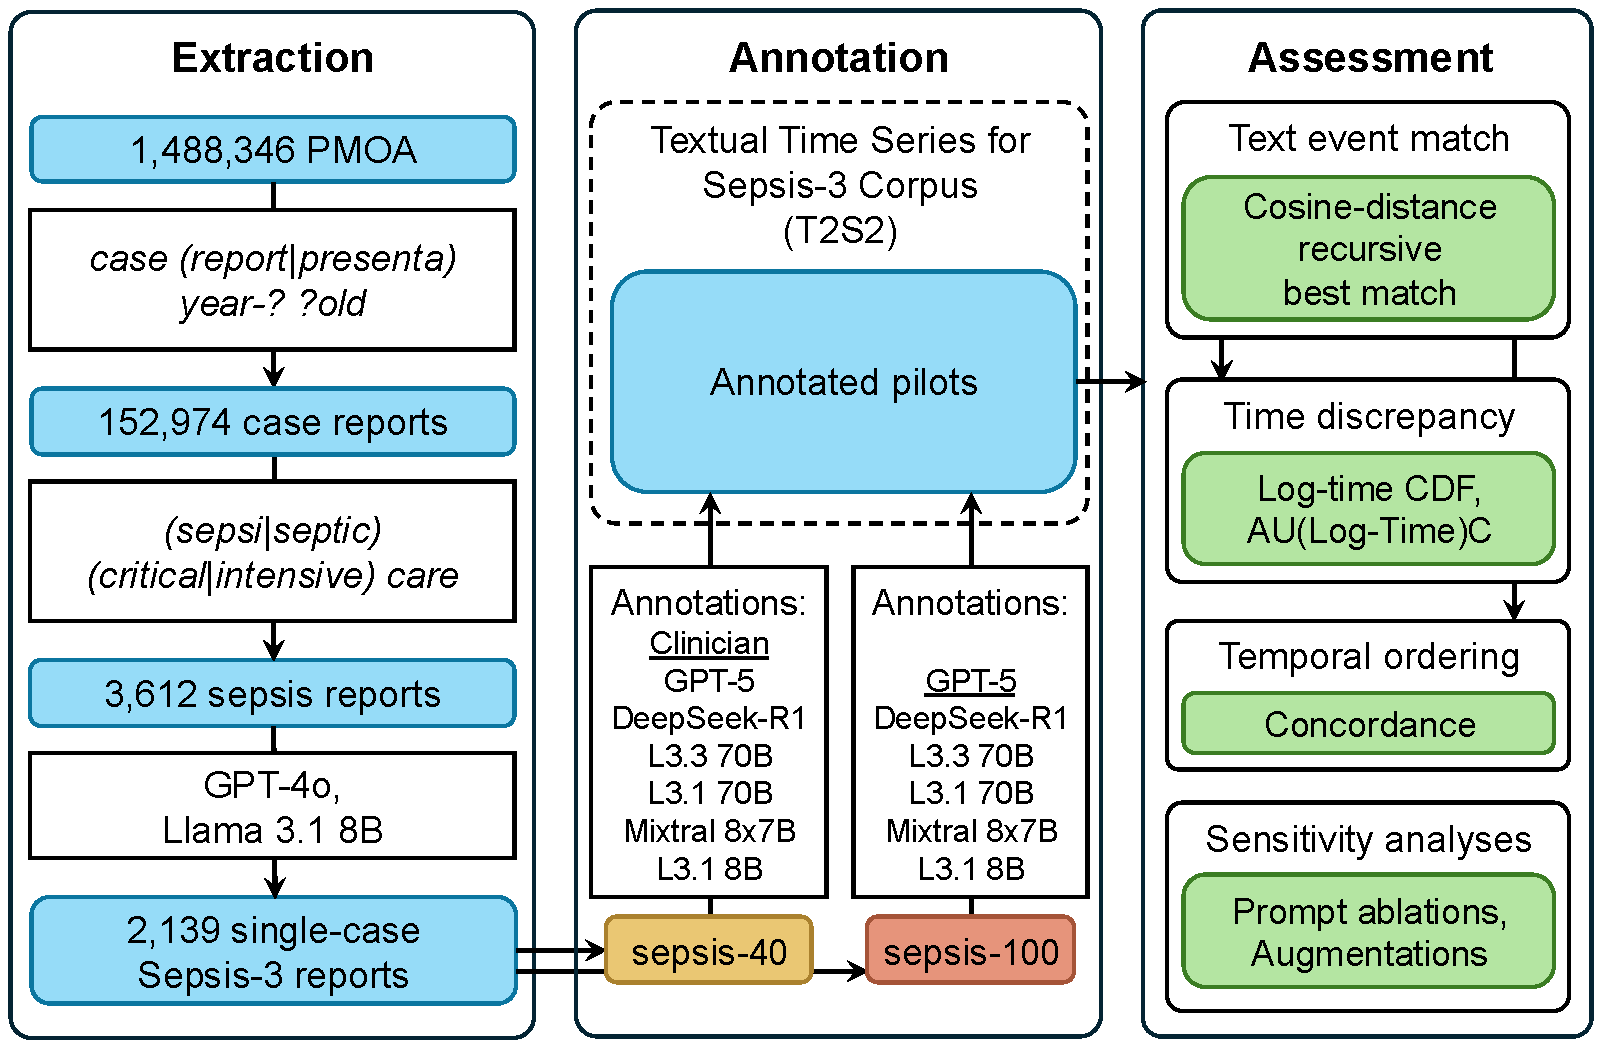
\includegraphics[width=\linewidth]{Chapters/chapter-05/sepsis/images/figures/T2S2-CHIL-Main-Figure.pdf}
  \end{minipage}%
  \hspace{.5em}
  \begin{minipage}[t]{0.30\textwidth}\vspace{0pt}
    \begin{adjustbox}{max width=\linewidth}\begin{tabular}{r|cc}
    \multicolumn{3}{c}{\textbf{i2m4}} \\
    \midrule
    Qwen\textbackslash Human & Yes & No \\
    Yes & 2 & 0 \\
    No  & 0 & 18 \\
    \toprule
    L3.1 8B & Yes & No \\
    Yes & 2 & 7 \\
    No  & 0 & 11 \\
    \midrule
    \multicolumn{3}{c}{\textbf{\texttt{sepsis-100}}} \\
    \toprule
    GPT-4o\textbackslash Qwen & Yes & No \\
    Yes & 78 & 7 \\
    No  & 8 & 7 \\
    \toprule
    L3.1 8B & Yes & No \\
    Yes & 81 & 12 \\
    No  & 5 & 2 \\
    \bottomrule
    \end{tabular}\end{adjustbox}
  \end{minipage}

  
  
  
  
\end{minipage}

\end{ChSixFloatBody}
\caption{Flowchart of the PMOA T2S2 corpus construction pipeline (left).
    Confusion matrices (right) for Sepsis-3 phenotype in i2m4 (top) and \texttt{sepsis-100} (bottom) datasets, with preferred annotator in column position.}\ChSixFloatLabel{ch06:fig:flow}
\end{figure}


\paragraph{Datasets}
\label{ch06:section:datasets}

\ChSixParagraph{i2m4.} This dataset contains 20 discharge summaries (15 i2b2, 5 MIMIC-IV) with physician-annotated temporal concepts from \cite{ch06:frattallone2024using}. We used interval lower bounds as event times and only probabilistic annotations. For Sepsis-3 phenotyping, we used a prompt describing qSOFA criteria: suspected/confirmed infection with blood pressure/respiratory rate/mental status abnormalities, requesting binary output (1 for sepsis, 0 otherwise).
To develop a computational approach, we used a prompt describing qSOFA criteria (Appendix \ref{ch06:apd:phenotype-prompt}) with QwQ-32B-Preview achieving 100\% accuracy and Llama-3.1-8B-Instruct achieving 65\% accuracy.

\ChSixParagraph{PMOA (\texttt{sepsis-40}, \texttt{sepsis-10}, \texttt{sepsis-100}).}
From 1.5M publications (source archive dated December 17, 2024), we identified case reports via regex (\texttt{case (report|presenta)} and \texttt{year-?old}), then filtered for sepsis using \texttt{(sepsi|septic)} and \texttt{(critical|intensive) care}.
GPT-4o and Llama-3.1-8B screened for Sepsis-3, yielding 2,139 cases.
We manually annotated 40 PMOA case reports for the gold-standard \texttt{sepsis-40} evaluation set, yielding $3,229$ clinician-annotated reference events.
The \texttt{sepsis-10} subset is a 10-report subset of \texttt{sepsis-40} used for clinician annotation quality review, hallucination audit, multi-pass self-consistency, and sepsis onset analysis.
We also sampled 100 non-overlapping PMOA case reports for \texttt{sepsis-100}, which is used as a bronze-standard proxy-reference set annotated by GPT-5 to evaluate extraction behavior at larger scale rather than as clinical ground truth.
The full case identifiers for \texttt{sepsis-40} and \texttt{sepsis-10} are provided in Appendix~\ref{ch06:apd:subset_ids}.
Figure~\ref{ch06:fig:flow} (right) shows phenotyping confusion matrices.

\textbf{Phenotyping output parsing and clinician audit.}
In practice, some LLMs produce verbose rationales rather than a minimal binary output.
We therefore parsed phenotyping decisions using a rule-based extraction step that searches model responses for explicit affirmative/negative indicators of meeting sepsis criteria and maps them to a binary label.
If primary extraction did not yield a valid label, a fallback strategy examined the final line of the response, and discordant parses were flagged for manual inspection.
We additionally performed clinician audit on sampled and borderline cases to verify alignment with Sepsis-3 intent under information available in narratives.


\paragraph{Clinical Finding Extraction and Temporal Assignment}
We define clinical findings with two key modifications from i2b2 clinical concepts \citep{ch06:uzuner20112010}: (1) findings extend beyond single prepositional phrases for specificity (e.g., ``pain in chest that radiates substernally'' remains intact), and (2) conjunctions split into components (e.g., ``metastases in liver and pancreas'' $\rightarrow$ \{``metastasis in liver'', ``metastasis in pancreas''\}).
Temporal assignment captures event start times (e.g., ``three-day history of fever'' $\rightarrow$ $t=-72$).
We queried six LLMs (GPT-5, DeepSeek-R1-UD-IQ1\_S, Llama-3.3-70B-Instruct, Llama-3.1-70B-Instruct, Mixtral-8x7B-Instruct v0.1, Llama-3.1-8B-Instruct) using a structured prompt with few-shot examples to extract event-time pairs.
The prompt instructs models to: assign admission time as $t=0$, use negative times for pre-admission events, split conjunctions, and capture event start times for durations (full prompt in Appendix \ref{ch06:apd:prompt}).
For sensitivity analysis, we tested ablations (no-role, zero-shot, no-expansion) and augmentations (interval bounds, i2b2 typing).

For i2m4, we compared against a BERT baseline adapted from \cite{ch06:frattallone2024using}, using a 3-layer MLP regressor with L1 loss for time prediction.
We filtered events to $\pm$2 weeks of admission for training stability (3,472$\rightarrow$3,350 findings) and used 5-fold cross-validation.

% !TeX root = ../../../../main.tex
\subsubsection{Evaluation Methodology}
\ChSixHeadingOnly
\paragraph{Quantitative evaluation of extracted timelines}
\label{ch06:sec:evaluation_methodology_metrics}
We evaluate extracted textual time series using four metrics:\\
\textbf{Event match rate}: Proportion of reference events matched via recursive best matching with cosine distance threshold 0.1 using PubMedBert embeddings (Appendix~\ref{ch06:apd:pseudo}).\\
\textbf{Concordance (c-index)}: Probability of correctly ordering random event pairs.\\
\textbf{Median absolute error (MAE)}: Median time discrepancy (in hours) among matched events.\\
\textbf{Area under log-time curve (AULTC)}: Integrated log-transformed discrepancies capturing accuracy across time scales (detailed derivation in Appendix \ref{ch06:apd:ltcdf}).

A clinician qualitative review of annotation quality on \texttt{sepsis-10} is described in Appendix~\ref{ch06:apd:clinician_quality_review}.





% !TeX root = ../../../../main.tex
\begin{table}[htbp]
\caption{Comparison of event match recall (Recall), median concordance ($c$), median absolute error (MAE), and area under the log-time curve (AULTC) across LLMs for i2m4, \texttt{sepsis-40}, and \texttt{sepsis-100} datasets.}\ChSixFloatLabel{ch06:tab:results}
\ChSixTableBodyStart
\begin{ChSixFloatBody}

\small


\footnotesize
\centering

\begin{adjustbox}{max width=\linewidth}\begin{tabular}{l*{12}{c}}
\toprule

& \multicolumn{4}{c}{i2m4}
& \multicolumn{4}{c}{\texttt{sepsis-40}}
& \multicolumn{4}{c}{\texttt{sepsis-100}} \\

\cmidrule(lr){2-5}
\cmidrule(lr){6-9}
\cmidrule(lr){10-13}

\textbf{Model}
& \scriptsize Recall
& \scriptsize c
& \scriptsize MAE
& \scriptsize AULTC
& \scriptsize Recall
& \scriptsize c
& \scriptsize MAE
& \scriptsize AULTC
& \scriptsize Recall
& \scriptsize c
& \scriptsize MAE
& \scriptsize AULTC \\

\midrule

GPT-5
& -- & -- & -- & --
& {\ChSixBfTab 0.93} & {\ChSixBfTab 0.965} & {\ChSixBfTab 4} & {\ChSixBfTab 0.822}
& -- & -- & -- & -- \\

DeepSeek-R1
& 0.31 & 0.755 & 13 & 0.786
& 0.79 & 0.892 & 16 & 0.781
& {\ChSixBfTab 0.77} & 0.879 & {\ChSixBfTab 2} & {\ChSixBfTab 0.812} \\

L3.3 70B
& {\ChSixBfTab 0.43} & {\ChSixBfTab 0.768} & {\ChSixBfTab 7} & {\ChSixBfTab 0.805}
& 0.76 & 0.908 & 24 & 0.742
& 0.69 & {\ChSixBfTab 0.920} & 7 & 0.796 \\

L3.1 70B
& 0.32 & 0.747 & 8 & 0.804
& 0.66 & 0.931 & 30 & 0.737
& 0.67 & 0.914 & 6 & 0.794 \\

Mixtral 8x7B
& 0.31 & 0.745 & 21 & 0.773
& 0.68 & 0.906 & 48 & 0.710
& 0.63 & 0.875 & 24 & 0.764 \\

L3.1 8B
& 0.35 & 0.727 & 26 & 0.738
& 0.53 & 0.856 & 84 & 0.685
& 0.66 & 0.772 & 50 & 0.716 \\

BERT 5-CV
& -- & 0.704 & 34 & 0.520
& -- & -- & -- & --
& -- & -- & -- & -- \\

\bottomrule
\end{tabular}\end{adjustbox}

\end{ChSixFloatBody}
\end{table}




% !TeX root = ../../../../main.tex
\subsubsection{Additional validation analyses}
\label{ch06:sec:additional_validation_methods}
We perform six additional validation analyses: (1) we quantify uncertainty on \texttt{sepsis-40} using document-level bootstrap resampling; (2) we measure inter-annotator agreement (IAA) on five additional case reports independently annotated by two clinicians; (3) using \texttt{sepsis-10}, we evaluate inference of sepsis onset timestamps from narratives (the onset inference prompt is provided in Appendix~\ref{ch06:apd:onset_prompt}); (4) using \texttt{sepsis-10}, we audit extracted events for hallucination by checking whether model-generated findings are grounded in the source report; (5) using the same \texttt{sepsis-10} reports, we evaluate multi-pass self-consistency by re-annotating reports under multiple random seeds; and (6) we estimate full-corpus cross-model agreement between DeepSeek-R1 and Llama-3.3-70B-Instruct across all 2,139 reports.
Detailed methods for the hallucination audit, self-consistency, and full-corpus agreement are provided in Appendix~\ref{ch06:apd:validation_details}.

\paragraph{Uncertainty quantification via document-level bootstrap (\texttt{sepsis-40})}
\label{ch06:sec:bootstrap_methods}

We use nonparametric bootstrap resampling at the \emph{case report} level with 200 bootstrap replicates.
In each replicate, we sample 40 case reports with replacement from \texttt{sepsis-40} and recompute event match rate, concordance, and AULTC.
We report percentile-based 95\% bootstrap confidence intervals.

\paragraph{Inter-annotator agreement on additional sepsis reports}
\label{ch06:sec:iaa_methods}
Two clinicians independently annotated five sampled T2S2 case reports using the same extraction and timestamping guidelines as \texttt{sepsis-40}.
We compute clinician--clinician agreement and model--clinician agreement using the same metrics (match rate, concordance, and AULTC), enabling comparison between model disagreement and human disagreement under the evaluation protocol.

\paragraph{Sepsis onset timestamp inference}
\label{ch06:sec:onset-inference}
In addition to extracting event--time pairs, we infer an explicit sepsis onset timestamp from narrative cues.
Given a case report, the onset procedure estimates the earliest time consistent with Sepsis-3 criteria relative to admission ($t=0$), producing two onset estimates based on qSOFA and SOFA-style reasoning when sufficient evidence is available.
We used GLM-4.6 (2-bit) for this inference.
The full prompt is provided in Appendix~\ref{ch06:apd:onset_prompt}.


\paragraph{Manual hallucination audit}
\label{ch06:sec:hallucination_audit_methods}
To directly evaluate whether extracted clinical findings were unsupported by the source text, we performed a two-stage hallucination audit on 10 sampled PMOA case reports.
We audited the DeepSeek-R1 and Llama-3.3-70B-Instruct outputs because they represent two strong model families used for corpus-scale annotation and agreement analyses.
First, we applied automated lexical grounding to each extracted event after light normalization, including removal of prompt-induced prefixes such as ``history of'' or ``treated with''.
The grounding step searched for exact substring matches, ordered token subsequences within a sentence, or unordered token containment in the source report.
Second, all events that could not be automatically grounded were manually reviewed against the original case report to determine whether they represented unsupported hallucinations or valid clinical transformations, such as abbreviation expansion, decomposition of conjunctions, or semantic paraphrasing.

\paragraph{Multi-pass self-consistency}
\label{ch06:sec:self_consistency_methods}
To assess robustness across generations, we re-annotated the same 10 reports used in the hallucination audit using five random seeds for DeepSeek-R1, Llama-3.3-70B-Instruct, OpenAI O1, and GPT-5.
For each model, Run 1 was treated as the within-model reference and Runs 2--5 were compared against it using the same event match rate, concordance, and AULTC metrics.
This analysis evaluates whether extracted timelines are stable across stochastic generations rather than being driven by isolated model-specific outputs.

\paragraph{Full-corpus cross-model agreement}
\label{ch06:sec:full_corpus_agreement_methods}
To estimate reliability beyond the human-annotated subset, we measured cross-model agreement between DeepSeek-R1 and Llama-3.3-70B-Instruct across the full 2,139-report T2S2 corpus.
We treated DeepSeek-R1 as the proxy reference and evaluated Llama-3.3-70B-Instruct using event match rate, concordance, and AULTC.
Because these models differ in architecture and training, agreement across the full corpus provides a scalable proxy for whether the extraction rules are applied consistently across independent model families.





% !TeX root = ../../../../main.tex
\subsection{Results}

In this section, we first detail the T2S2 corpus and phenotyping accuracy, then evaluate LLM-extracted timelines against clinician annotations and bronze-standard proxy references.
We then present additional validation analyses addressing uncertainty, annotator variability, sepsis onset inference, factual grounding, self-consistency, and full-corpus agreement.



% !TeX root = ../../../../main.tex
\subsubsection{Corpus overview}

Our analysis resulted in T2S2, a new open-access textual time series corpus for Sepsis-3\footnote{Sepsis-3 refers to the Third International Consensus Definitions for Sepsis and Septic Shock \citep{singer2016third}, which define sepsis as a life-threatening organ dysfunction caused by a dysregulated host response to infection.
In contrast, \texttt{sepsis-40}, \texttt{sepsis-10}, and \texttt{sepsis-100}, introduced in this paper, refer to subsets of sepsis reports drawn from PMOA, with the numbers indicating the subset size.}, 
comprising 2,139 case reports.  
Demographically, the corpus includes 58\% male and 42\% female patients, with ages ranging from 0 to 111 and a mean age of 49 (IQR: 32--65).

% !TeX root = ../../../../main.tex
\subsubsection{Phenotyping Results}
For phenotyping the i2m4 dataset for sepsis, we found two case reports of patients with sepsis.
The QwQ-32B-Preview response had perfect accuracy (100\%), whereas the Llama-3.1-8B-Instruct accuracy was 13/20 (65\%).
For the \texttt{sepsis-100} dataset, where QwQ-32B-Preview outputs were used as the preferred computational labels, the relatively faster models GPT-4o and Llama-3.1-8B-Instruct agreed 84\% and 83\% of the time, respectively (Figure~\ref{ch06:fig:flow}, bottom right).
Although QwQ-32B-Preview sometimes produced verbose rationales that referenced SOFA-style reasoning, the operational phenotyping decision was mapped to the requested binary output using the rule-based parsing and clinician-audit process described in Section~\ref{ch06:section:datasets}.
We therefore interpret these phenotyping labels as cohort-selection outputs for constructing a retrospective research corpus, rather than as a primary clinical phenotyping benchmark.


% !TeX root = ../../../../main.tex
\subsubsection{Evaluation of Textual Time Series Corpus for Sepsis}
\ChSixHeadingOnly
\paragraph{Quantitative evaluation of extracted annotations}
\label{ch06:sec:annotation_results_quantitative}
Following the quantitative evaluation protocol described in Section~\ref{ch06:sec:evaluation_methodology_metrics}, Table~\ref{ch06:tab:results} reports performance across i2m4, \texttt{sepsis-40}, and \texttt{sepsis-100}.

% !TeX root = ../../../../main.tex
\begin{table}[htbp]
\caption{Comparison of event match recall (Recall), median concordance ($c$), median absolute error (MAE), and area under the log-time curve (AULTC) across LLMs for i2m4, \texttt{sepsis-40}, and \texttt{sepsis-100} datasets.}\ChSixFloatLabel{ch06:tab:results}
\ChSixTableBodyStart
\begin{ChSixFloatBody}

\small


\footnotesize
\centering

\begin{adjustbox}{max width=\linewidth}\begin{tabular}{l*{12}{c}}
\toprule

& \multicolumn{4}{c}{i2m4}
& \multicolumn{4}{c}{\texttt{sepsis-40}}
& \multicolumn{4}{c}{\texttt{sepsis-100}} \\

\cmidrule(lr){2-5}
\cmidrule(lr){6-9}
\cmidrule(lr){10-13}

\textbf{Model}
& \scriptsize Recall
& \scriptsize c
& \scriptsize MAE
& \scriptsize AULTC
& \scriptsize Recall
& \scriptsize c
& \scriptsize MAE
& \scriptsize AULTC
& \scriptsize Recall
& \scriptsize c
& \scriptsize MAE
& \scriptsize AULTC \\

\midrule

GPT-5
& -- & -- & -- & --
& {\ChSixBfTab 0.93} & {\ChSixBfTab 0.965} & {\ChSixBfTab 4} & {\ChSixBfTab 0.822}
& -- & -- & -- & -- \\

DeepSeek-R1
& 0.31 & 0.755 & 13 & 0.786
& 0.79 & 0.892 & 16 & 0.781
& {\ChSixBfTab 0.77} & 0.879 & {\ChSixBfTab 2} & {\ChSixBfTab 0.812} \\

L3.3 70B
& {\ChSixBfTab 0.43} & {\ChSixBfTab 0.768} & {\ChSixBfTab 7} & {\ChSixBfTab 0.805}
& 0.76 & 0.908 & 24 & 0.742
& 0.69 & {\ChSixBfTab 0.920} & 7 & 0.796 \\

L3.1 70B
& 0.32 & 0.747 & 8 & 0.804
& 0.66 & 0.931 & 30 & 0.737
& 0.67 & 0.914 & 6 & 0.794 \\

Mixtral 8x7B
& 0.31 & 0.745 & 21 & 0.773
& 0.68 & 0.906 & 48 & 0.710
& 0.63 & 0.875 & 24 & 0.764 \\

L3.1 8B
& 0.35 & 0.727 & 26 & 0.738
& 0.53 & 0.856 & 84 & 0.685
& 0.66 & 0.772 & 50 & 0.716 \\

BERT 5-CV
& -- & 0.704 & 34 & 0.520
& -- & -- & -- & --
& -- & -- & -- & -- \\

\bottomrule
\end{tabular}\end{adjustbox}

\end{ChSixFloatBody}
\end{table}

On the clinician-annotated \texttt{sepsis-40} set, GPT-5 is the strongest annotator across all four metrics, with event match recall 0.93, concordance 0.965, median absolute error 4 hours, and AULTC 0.822.
DeepSeek-R1 provides the next strongest overall performance on \texttt{sepsis-40}, with higher event recovery and AULTC than Llama 3.3 (event match recall 0.79 vs.\ 0.76; AULTC 0.781 vs.\ 0.742), whereas Llama 3.1 70B and Llama 3.3 show high concordance among their matched events.
This pattern highlights a recurring tradeoff in the evaluation: models can achieve high temporal ordering among the subset of events they match, while still recovering fewer reference events or producing larger absolute timestamp discrepancies.

The i2m4 results should be interpreted as a cross-schema evaluation rather than a direct in-domain test of T2S2-style extraction.
All LLM event match recall values are lower on i2m4, where the reference annotations are legacy i2b2-style temporal concepts rather than standalone clinical findings.
Among the LLMs, Llama 3.3 performs best on i2m4 across event match recall, concordance, median absolute error, and AULTC, and all LLMs with temporal predictions substantially outperform the BERT 5-CV time-regression baseline on AULTC.
However, the low event match recall values indicate that many clinically meaningful T2S2-style findings are penalized when compared against fragmented concept-level references.
In contrast to concordances around 0.76 in i2m4, in \texttt{sepsis-40}, GPT-5 and Llama 3.3 were excellent time-ordering annotators, with concordances of 0.965 and 0.908, respectively.

On \texttt{sepsis-100}, which is a bronze-standard proxy-reference set rather than clinical ground truth, DeepSeek-R1 achieves the highest event match recall, lowest median absolute error, and highest AULTC against the GPT-5 reference, while Llama 3.3 achieves the highest concordance.
These results should therefore be read as scalable proxy-reference evaluation of extraction behavior, not as an estimate of absolute clinical accuracy.

\paragraph{Uncertainty quantification via document-level bootstrap (\texttt{sepsis-40})}
Because clinician-annotated evaluation sets are necessarily limited in size, we quantify uncertainty using nonparametric bootstrap resampling at the \emph{case report} level with 200 bootstrap replicates.
In each replicate, we sample 40 case reports with replacement from \texttt{sepsis-40} and recompute event match recall, concordance, and AULTC.
We report percentile-based 95\% bootstrap confidence intervals.
Table~\ref{ch06:tab:bootstrap_ci} summarizes these intervals.
Across models, the bootstrap intervals preserve the main qualitative conclusions from Table~\ref{ch06:tab:results}: GPT-5 is the strongest model on \texttt{sepsis-40}, DeepSeek-R1 and Llama 3.3 remain the strongest open-model annotators overall, and the smaller or older models generally show lower event recovery and/or temporal accuracy.


% !TeX root = ../../../../main.tex
\begin{table}[htbp]
\caption{Case report bootstrap 95\% confidence intervals (CIs) on \texttt{sepsis-40}. The bootstrap resamples \emph{case reports} with replacement and recomputes metrics per replicate.}\ChSixFloatLabel{ch06:tab:bootstrap_ci}
\ChSixTableBodyStart
\begin{ChSixFloatBody}

\centering
\small


\adjustbox{max width=\columnwidth}{
\begin{tabular}{lccc}
\toprule
Model & Event match recall & Concordance & AULTC \\
\midrule
GPT-5 & [0.879, 0.930] & [0.956, 0.977] & [0.775, 0.863] \\
DeepSeek-R1 & [0.742, 0.840] & [0.846, 0.929] & [0.724, 0.825] \\
L3.3 70B & [0.731, 0.800] & [0.881, 0.936] & [0.704, 0.790] \\
L3.1 70B & [0.606, 0.705] & [0.897, 0.950] & [0.695, 0.787] \\
Mixtral 8x7B & [0.616, 0.743] & [0.817, 0.935] & [0.667, 0.765] \\
L3.1 8B & [0.483, 0.591] & [0.826, 0.898] & [0.634, 0.736] \\
\bottomrule
\end{tabular}
}

\end{ChSixFloatBody}
\end{table}


To better understand the performance differences across datasets, we conducted an error analysis between \texttt{sepsis-10} and i2m4, presented in Appendix~\ref{ch06:apd:error-analysis}.
This analysis shows that the i2m4 performance gap is driven in part by annotation-ontology mismatch between fragmented i2b2 concepts and the more compositional clinical findings targeted by T2S2.



% !TeX root = ../../../../main.tex
\begin{table}[htbp]
\caption{Comparison of event match recall (Recall), median concordance ($c$), median absolute error (MAE), and area under the log-time curve (AULTC) across Llama-3.3-70B-Instruct prompt variants: no role-playing (no role), no conjunction expansion (no expansion), zero-shot, interval, and interval with i2b2 event typing (Interval + Type), for i2m4, \texttt{sepsis-40}, and \texttt{sepsis-100}.}\ChSixFloatLabel{ch06:tab:sens}
\ChSixTableBodyStart
\begin{ChSixFloatBody}

\scriptsize


\footnotesize
\centering

\begin{adjustbox}{max width=\linewidth}\begin{tabular}{l*{12}{c}}
\toprule

& \multicolumn{4}{c}{i2m4}
& \multicolumn{4}{c}{\texttt{sepsis-40}}
& \multicolumn{4}{c}{\texttt{sepsis-100}} \\

\cmidrule(lr){2-5}
\cmidrule(lr){6-9}
\cmidrule(lr){10-13}

\textbf{Model}
& \scriptsize Recall
& \scriptsize c
& \scriptsize MAE
& \scriptsize AULTC
& \scriptsize Recall
& \scriptsize c
& \scriptsize MAE
& \scriptsize AULTC
& \scriptsize Recall
& \scriptsize c
& \scriptsize MAE
& \scriptsize AULTC \\

\midrule

L3.3 70B
& {\ChSixBfTab 0.43} & 0.768 & {\ChSixBfTab 7} & {\ChSixBfTab 0.805}
& {\ChSixBfTab 0.76} & 0.908 & 24 & 0.742
& 0.69 & 0.920 & 7 & {\ChSixBfTab 0.796} \\
\\

\textbf{Ablations} \\
No role
& 0.40 & 0.734 & 8 & 0.800
& 0.75 & 0.920 & 24 & 0.749
& 0.69 & 0.908 & 8 & 0.792 \\

No expansion
& 0.38 & 0.768 & 8 & 0.797
& 0.76 & 0.909 & 24 & {\ChSixBfTab 0.774}
& 0.69 & 0.923 & 7 & 0.795 \\

Zero-shot
& 0.30 & 0.737 & 9 & 0.794
& 0.64 & {\ChSixBfTab 0.940} & 24 & 0.746
& 0.59 & {\ChSixBfTab 0.943} & 12 & 0.786 \\
\\

\textbf{Augments} \\
Interval
& 0.43 & 0.740 & 8 & 0.798
& 0.74 & 0.924 & 24 & 0.737
& {\ChSixBfTab 0.70} & 0.902 & 10 & 0.789 \\

Interval+Type
& 0.39 & {\ChSixBfTab 0.775} & 8 & 0.803
& 0.71 & 0.911 & 28 & 0.730
& 0.68 & 0.906 & {\ChSixBfTab 6} & 0.794 \\

\bottomrule
\end{tabular}\end{adjustbox}

\end{ChSixFloatBody}
\end{table}



To examine the results in greater detail, we show figures of the cumulative distribution function of event matches and concordance boxplots (Figure \ref{ch06:fig:time-disc}) for the \texttt{sepsis-40} dataset.
When the function reaches its maximum at the maximum cosine distance, it may be less than 1 because the label events have no events left to match, \emph{i.e.}, the reference method recovered an event that the prediction method did not.
The event match recall values in Table \ref{ch06:tab:results} correspond to the event match recall at the cosine distance threshold in Figure \ref{ch06:fig:time-disc} ($\theta=0.10$).
One could adjust the cosine distance threshold, for example, by increasing it to increase matches, at the cost of false positive matches that degrade temporal performance.
We provide a systematic threshold analysis over $\theta \in [0.01, 0.5]$ in 0.01 increments in Appendix~\ref{ch06:apd:threshold_sweep}, which demonstrates a clear elbow near $\theta=0.10$ and supports our chosen operating point.
The concordance box plots (Figure \ref{ch06:fig:time-disc}) show strong performance among the large LLMs, whereas the Llama 3.1 8B and Mixtral 8x7B model performances are much lower, which is a consistent finding throughout our analysis.

To better visualize timestamp discrepancies, we plot cumulative time-discrepancy curves among matched events (Figure~\ref{ch06:fig:time-disc}).
GPT-5 has the strongest overall time-discrepancy profile, consistent with its median absolute error of 4 hours and highest AULTC in Table~\ref{ch06:tab:results}.
The disaggregated curves further show that near-admission events are easier to timestamp than events occurring months or years away from presentation.
This degradation at longer horizons is consistent with the expert qualitative review, which identified ambiguity for events with extended duration and errors in cases requiring chained relative-time reasoning (Appendix~\ref{ch06:apd:clinician_quality_review}).
This long-horizon degradation is most visible in the bottom subpanels of Figure~\ref{ch06:fig:time-disc} (right), where the strongest models recover a larger fraction of distant events within the correct coarse time scale.

\ChSixParagraph{Sensitivity analysis of prompt components.}
The sensitivity analysis to our chosen prompt shows that prompt components affect event recovery and temporal metrics in different ways for Llama-3.3-70B-Instruct (Table~\ref{ch06:tab:sens}).
The full prompt remains a strong and balanced operating point, especially for i2m4, where it obtains the highest event match recall, lowest median absolute error, and highest AULTC.
On \texttt{sepsis-40}, removing conjunction expansion preserves the event match recall and improves AULTC, while zero-shot prompting yields higher concordance among matched events but substantially reduces event recovery.
This suggests that high concordance alone can be misleading when fewer or easier-to-order events are matched.
The interval and interval+type augmentations do not consistently improve performance: interval prompting slightly increases event match recall on \texttt{sepsis-100}, but not on \texttt{sepsis-40}, and the additional type field generally does not improve the overall balance of event recovery and temporal accuracy.
Together, these results indicate that adding output fields can increase prompt burden and does not necessarily improve the quality of the extracted textual time series across the models used.




% !TeX root = ../../../../main.tex
\begin{figure}[htbp]
\begin{ChSixFloatBody}

    \begin{minipage}[t]{0.24\textwidth}
    \centering
    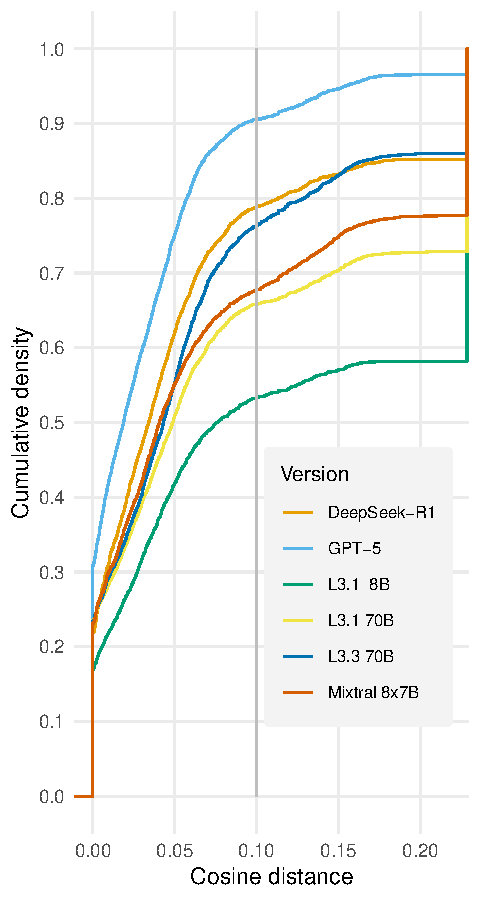
\includegraphics[width=\linewidth, page=1]{Chapters/chapter-05/sepsis/images/figures/main_results_figures/figures_sepsis_40.pdf}
    \end{minipage}
    \hfill
    \begin{minipage}[t]{0.24\textwidth}
    \centering
    \includegraphics[width=\linewidth, page=2]{Chapters/chapter-05/sepsis/images/figures/main_results_figures/figures_sepsis_40.pdf}
    \end{minipage}
    \begin{minipage}[t]{0.24\textwidth}
    \centering
    \includegraphics[width=\linewidth, page=3]{Chapters/chapter-05/sepsis/images/figures/main_results_figures/figures_sepsis_40.pdf}
    \end{minipage}
    \begin{minipage}[t]{0.24\textwidth}
    \centering
    \includegraphics[width=\linewidth, page=4]{Chapters/chapter-05/sepsis/images/figures/main_results_figures/figures_sepsis_40.pdf}
    \end{minipage}
    
    
    

\end{ChSixFloatBody}
\caption{Event match cumulative distribution function (left), concordance box-plots (middle left), 
    time discrepancy from the manual annotation timestamps among matched events, overall (middle right), and disaggregated by clinician annotator timestamp (time from presentation, right) for the \texttt{sepsis-40} dataset.}\ChSixFloatLabel{ch06:fig:time-disc}
\end{figure}

% !TeX root = ../../../../main.tex
\subsection{Clinical Reliability, Validation, and Error Analysis}
\label{ch06:sec:additional_validation}

\ChSixHeadingOnly

\subsubsection{Inter-annotator Agreement}
\label{ch06:sec:iaa}
To contextualize residual model--clinician discrepancies, we quantified agreement between two independent clinician annotators on five sampled case reports from T2S2, annotated under the same guidelines.
We report (i) model--annotator alignment for two leading LLM annotators against each clinician and (ii) clinician--clinician agreement using the same metrics as the main evaluation.


% !TeX root = ../../../../main.tex
\begin{table}[htbp]
\caption{Inter-annotator agreement across reports.}\ChSixFloatLabel{ch06:tab:iaa_manual}
\ChSixTableBodyStart
\begin{ChSixFloatBody}

\centering
\small


\begin{adjustbox}{max width=\columnwidth}
\begin{tabular}{lccc}
\toprule
Annotator pair & Recall & Concordance & AULTC \\
\midrule
A1 vs.\ A2 (Manual) & 0.681 & 0.912 & 0.811 \\
\bottomrule
\end{tabular}
\end{adjustbox}

\end{ChSixFloatBody}
\end{table}







Tables~\ref{ch06:tab:iaa_manual} and~\ref{ch06:tab:iaa_models} contextualize the main results by quantifying annotator variability under the same guidelines and metrics.
Clinician--clinician agreement is imperfect even on the same case reports (Table~\ref{ch06:tab:iaa_manual}), reflecting inherent ambiguity in mapping narrative descriptions to temporally localized findings and timestamps.
Against this reference, the strongest LLM annotators achieve model--clinician agreement that is comparable to clinician--clinician agreement across the same metrics (Table~\ref{ch06:tab:iaa_models}), supporting that the leading performance levels in Table~\ref{ch06:tab:results} are meaningful relative to human variability rather than artifacts of the evaluation protocol.

\paragraph{Inter-annotator agreement on a GLP1-RA subset}
\label{ch05:glp_iaa}

\ChFiveRebuttal{To contextualize agreement with the single-expert reference set, we also analyzed a separate 140-case report subset of PMOA-TTS involving patients who took GLP-1 RA (Glucagon-like Peptide Receptor Agonists) medications. Two clinically trained annotators independently constructed event-time timelines for this subset using the same annotation framework. Using Annotator 1 as the reference and the same matching and temporal metrics used for the model evaluation, Annotator 2 achieved an event match recall of 0.811, temporal concordance of 0.798, and AULTC of 0.702.}

% !TeX root = ../../../../main.tex

\subsubsection{Clinician Annotation Quality Review}

A clinician qualitative review of annotation quality on \texttt{sepsis-10} is described in Appendix~\ref{ch06:apd:clinician_quality_review}.

The reviewed annotation bundle included O1-preview as the OpenAI annotation; replacing GPT-5 which was evaluated separately in the main quantitative results in Table~\ref{ch06:tab:results}.

Inspecting the clinical quality of the annotations, we report the mean rank, top-1 fraction, top-1-LLM fraction, and quality level in Table~\ref{ch06:tab:sep10review}.
There is a clear performance ordering in the review, with manual annotations ranked highest, O1-preview a close second, followed by DeepSeek-R1 IQ1 and Llama 3.3.
While the Llama 3.3 annotations were rated acceptable a high percentage of the time (90\%), the other Llama and Mixtral approaches fail to achieve Acceptable performance in excess of 50\%.
Comparing DeepSeek-R1 IQ1 and Llama 3.3, the former has more variable clinician-rated quality (8 of 10 cases rated Acceptable or better), but maintains both higher event match recall and AULTC in the main quantitative evaluation (Table~\ref{ch06:tab:results} and Figure~\ref{ch06:fig:time-disc}).
The clinical reviewer also noted that some Llama 3.3 discrepancies for large time horizons, \emph{i.e.}, years, were large, which is corroborated by the long-horizon subpanels in Figure~\ref{ch06:fig:time-disc}.

% !TeX root = ../../../../main.tex
\begin{table}[htbp]
\caption{Clinician annotation quality review on \texttt{sepsis-10}.}\ChSixFloatLabel{ch06:tab:sep10review}
\ChSixTableBodyStart
\begin{ChSixFloatBody}

\centering
\small


\begin{tabular}{lcccccc}
\toprule
Annotator & Mean Rank & Top-1 & Top-1-LLM & Excellent & $\geq$ Good & $\geq$ Acceptable \\
\midrule
Manual & 1.2 & 0.9 & -- & 1 & 1 & 1 \\
O1-preview & 1.5 & 0.6 & 0.9 & 0.9 & 1 & 1 \\
DeepSeek R1 IQ1 & 3.5 & 0.1 & 0.2 & 0.4 & 0.5 & 0.8 \\
L3.3 70B & 3.8 & 0 & 0 & 0 & 0.2 & 0.9 \\
L3.1 70B & 4.8 & 0 & 0 & 0 & 0.2 & 0.5 \\
Mixtral 8x7B & 5.4 & 0 & 0 & 0 & 0.1 & 0.2 \\
L3.1 8B & 6.5 & 0 & 0 & 0 & 0 & 0 \\
\bottomrule
\end{tabular}

\end{ChSixFloatBody}
\end{table}


\subsubsection{Sepsis Onset Timestamp Inference}
\label{ch06:sec:onset-inference}
In addition to extracting event--time pairs, we infer an explicit sepsis onset timestamp from narrative cues.
Given a case report, the onset procedure estimates the earliest time consistent with Sepsis-3 criteria relative to admission ($t=0$), producing two onset estimates based on qSOFA and SOFA-style reasoning when sufficient evidence is available.
We used GLM-4.6 (2-bit) for this inference.
The full prompt is provided in Appendix~\ref{ch06:apd:onset_prompt}.

\label{ch06:sec:onset_results}

On \texttt{sepsis-10}, SOFA-based onset matched clinician onset exactly in 6 of 9 valid cases where onset could be assessed, excluding one neonatal outlier for which neonatal SOFA would be more appropriate.
The median absolute error was 0 hours (mean $\approx 3.4$ hours), with a single moderate deviation of 24 hours.
In contrast, qSOFA-based onset tended to lag substantially (mean absolute error $\approx 355$ hours including the outlier and $\approx 126$ hours excluding it), consistent with retrospective reporting of qSOFA-related cues in case narratives rather than true physiologic delay, whereas SOFA-based onset closely aligned with clinician-annotated sepsis onset.

\subsubsection{Grounding and Consistency}
\label{ch06:sec:additional_validation_summary}

We further evaluated factual grounding, generation stability, and full-corpus consistency using analyses summarized here and detailed in Appendix~\ref{ch06:apd:validation_details}.
In the \texttt{sepsis-10} hallucination audit, 1,517 total extracted events from combined DeepSeek-R1 and Llama-3.3-70B-Instruct were reviewed through automated lexical grounding followed by manual adjudication of unresolved cases; no unsupported hallucinated events were identified (Table~\ref{ch06:tab:hallucination_audit} in Appendix~\ref{ch06:apd:hallucination_audit_results}).
On the same \texttt{sepsis-10} reports, multi-pass self-consistency across five random seeds showed stable extraction behavior across DeepSeek-R1, Llama 3.3, O1-preview, and GPT-5 (Table~\ref{ch06:tab:self_consistency} in Appendix~\ref{ch06:apd:self_consistency_results}).
Across the full 2,139-report corpus, Llama-3.3-70B-Instruct achieved strong agreement with DeepSeek-R1, with event match recall 0.79, concordance 0.87, and AULTC 0.83 (Table~\ref{ch06:tab:full_corpus_agreement} in Appendix~\ref{ch06:apd:full_corpus_agreement_results}).

\subsubsection{Annotation Error Analysis}
We qualitatively compared temporal annotations produced by several LLMs on a representative case report to illustrate characteristic differences in event extraction and timestamping (Supplementary Material, Section~\ref{ch05:apd:inter-llm-comparison}).
While all models recovered the major clinical trajectory and preserved temporal polarity, they varied in
event granularity, paraphrasing, and long-range temporal normalization.
These differences complement the aggregate quantitative results and highlight the impact of model behavior on the structure of extracted timelines.
Common model-specific error patterns, such as granularity variation, duplicate events, and differences in temporal normalization, are summarized in the Supplementary Material, Section~\ref{ch05:apd:inter-llm-comparison}, Table~\ref{ch05:tab:error_taxonomy}.

% !TeX root = ../../../../main.tex
\subsection{Discussion and Conclusions}
We developed an analytical pipeline for processing free-text biomedical case reports into Sepsis-3 textual time series using large language models.
The resulting T2S2 corpus contains 2,139 open-access PMOA case reports represented as event--timestamp trajectories, providing a retrospective resource for temporal modeling of sepsis narratives.
Evaluation on the clinician-annotated \texttt{sepsis-40} subset shows strong performance, with GPT-5 achieving the strongest overall results and DeepSeek-R1 and Llama 3.3 providing competitive open-model baselines with different tradeoffs across event recovery, temporal ordering, and absolute timestamp accuracy. 
Additional analyses, including document-level bootstrapping, clinician--clinician agreement, sepsis onset inference, hallucination auditing, self-consistency evaluation, and cross-model agreement on \texttt{sepsis-100} and the full corpus, further contextualize the reliability and limitations of the extracted trajectories.
These results support T2S2 as a retrospective research corpus for downstream tasks such as risk forecasting, causal reasoning, and disease trajectory characterization, while making clear that it is not intended as a deployment-ready clinical extraction system.


There are several limitations to our work.
First, T2S2 is a clinical research informatics corpus constructed from published case reports and should not be considered a representative sample of all patients with sepsis.
Case report corpora are affected by publication bias, rare finding over-representation, selective reporting, and retrospective revisionism.
The corpus is therefore best suited for studying retrospective sepsis trajectories, developing temporal modeling methods, and analyzing narrative representations, rather than estimating population-level incidence or deployment-ready clinical performance.

Second, while \texttt{sepsis-40} provides a substantially expanded human gold standard, exhaustive clinician validation of the full 2,139-report corpus remains infeasible.
The additional validation analyses reduce but do not eliminate this limitation: hallucination auditing provides direct evidence of factual grounding in a sampled subset, self-consistency evaluates stability across repeated generations, and full-corpus cross-model agreement assesses reproducibility across model families.
However, these analyses do not replace clinician adjudication of every extracted event.
A complete characterization of corpus-wide errors would require a larger human-in-the-loop adjudication framework in which clinicians resolve model disagreements and temporal ambiguities.

Third, the substantial use of LLMs in the analytic pipeline can make error analysis difficult because errors may be subtle, clinically plausible, or concentrated in ambiguous temporal expressions.
Our hallucination audit suggests that unsupported event fabrication is uncommon in the audited subset under the extractive formulation, but timestamp errors remain possible even when the event itself is text-grounded.
This distinction is important: the primary failure mode in this task is often not hallucinating a clinical finding, but assigning the wrong time to a real finding, especially when timing requires chained relative reasoning or interpretation of vague duration phrases.

Fourth, the i2m4 analysis should be interpreted as a cross-schema evaluation.
The lower event match rates on i2m4 arise in part from mismatch between fragmented i2b2-style temporal concepts and T2S2-style standalone clinical findings.
For example, section headers, isolated abbreviations, or partial phrases can appear as i2b2 concepts, whereas the T2S2 representation intentionally favors clinically meaningful, compositional findings.
This means that i2m4 is useful as a legacy benchmark and stress test, but it is not a clean estimate of T2S2 extraction performance on clinical notes without re-annotation under the T2S2 schema.

While T2S2 provides a retrospective resource for studying sepsis trajectories, translating this pipeline into a prospective clinical tool would require a different extraction architecture.
Real-time clinical documentation is substantially noisier than finalized case reports or retrospective discharge summaries, and the available information changes continuously as care unfolds.
A prospective system would need to process note updates incrementally, integrate extracted textual findings with streaming structured EHR data such as vitals and laboratory results, calibrate predictions against prospective clinical outcomes, and evaluate safety under deployment-specific error modes.
Until such bridging work is completed, T2S2 should be viewed as a high-fidelity retrospective resource for temporal modeling and clinical trajectory analysis rather than as a clinical decision-support system.

Regarding generalizability to other medical conditions besides sepsis, our methodology could be extended in a straightforward manner.
Our motivation for choosing sepsis as the disease focus was to expand the analysis from the i2m4 dataset to a similar population in the PMOA corpus and maintain a well-defined phenotype.
Sepsis is a sensible choice as it is one of the most prevalent and important diagnoses in critical care medicine.  
However, there are several concerns when generalizing to other conditions.
For one, most other conditions are less acute in nature, meaning that the time distributions may be wider.
Also, the amount and type of information in such case reports may vary. 
Despite this, one benefit of AULTC compared to linear or squared discrepancies is that when intensive-care and chronic-disease cases are mixed, long-horizon discrepancies from chronic disease cases do not dominate the performance measure because of the log-time scaling.
Another generalizability concern is that for some conditions, less temporal information will be present.
This appears to be more acute in imaging studies, where the focus of the case is on the image content at a single snapshot in time.
For these types of studies, the longitudinal annotations become less meaningful compared to the image's information content.

Future work could focus on expanding this methodological framework.
While our current prompt augmentations did not yield systematic performance gains (Table \ref{ch06:tab:sens}), exploring advanced prompting paradigms alongside domain-specific fine-tuning could further refine the fidelity and expressivity of the extracted representations.
We anticipate that T2S2 will serve as a foundational resource for downstream healthcare applications, including causal inference, risk forecasting, and multimodal alignment.
The empirical utility of this representation is evidenced by our concurrent work, which leverages T2S2 from clinical narratives to accurately forecast future patient risk states \citep{noroozizadeh2026forecasting}.
Ultimately, advancing temporal AI in healthcare requires exploiting all available modalities; the extraction of structured temporal trajectories from narrative text provides a critical complement to existing structured data streams.

Subsequent iterations of this pipeline can be tailored to specific downstream objectives, each imposing distinct constraints.
For instance, causal modeling requires strict time-ordering, whereas forecasting demands precise absolute timestamps.
Furthermore, while our current formulation targets true physiological occurrence, an alternative paradigm could focus on the timing of clinical recognition.
Capturing these perceived occurrences could illuminate decision-making dynamics and facilitate research in dynamic resource allocation. 
Ultimately, integrating these narrative-derived timelines with structured physiological data offers a promising avenue to build more comprehensive, multimodal representations of patient trajectories.



% % !TeX root = ../../../../main.tex

\ChSixAcknowledgments{
This research was supported in part by the Division of Intramural Research (DIR) of the National Library of Medicine (NLM), National Institutes of Health.
This work utilized the computational resources of the NIH HPC Biowulf cluster.
S.N. was supported by Carnegie Mellon University TCS Presidential Fellowship, and Natural Sciences and Engineering Research Council of Canada (NSERC) Canada Graduate Research Scholarship --- Doctoral (CGRS D). S.N. was also supported in part by an appointment to the National Library of Medicine Research Participation Program administered by the Oak Ridge Institute for Science and Education (ORISE) through an interagency agreement between the U.S. Department of Energy (DOE) and the National Library of Medicine, National Institutes of Health. ORISE is managed by ORAU under DOE contract number DE-SC0014664. All opinions expressed in this paper are the authors’ and do not necessarily reflect the policies and views of NIH, NLM, DOE, or ORAU/ORISE.}


\clearpage
\endgroup
